\documentclass[conference]{IEEEtran}
\IEEEoverridecommandlockouts
\usepackage{cite}
\usepackage{amsmath,amssymb,amsfonts}
\usepackage{algorithmic}
\usepackage{graphicx}
\usepackage{textcomp}
\usepackage{xcolor}
\usepackage{hyperref}
\usepackage{listings}
\usepackage{tabularx}
\usepackage{balance}

\newcolumntype{C}{>{\centering\arraybackslash}X}

\usepackage{tikz}
\usetikzlibrary{shapes,arrows,positioning,fit,backgrounds}

\def\BibTeX{{\rm B\kern-.05em{\sc i\kern-.025em b}\kern-.08em
    T\kern-.1667em\lower.7ex\hbox{E}\kern-.125emX}}

\lstset{
  basicstyle=\ttfamily\scriptsize,
  columns=fullflexible,
  frame=single,
  breaklines=true,
  captionpos=b,
}

\begin{document}

\title{Secure-by-Default Guardrails for MCP-Based Tool Use in Multi-Modal LLM Agents}

\author{\IEEEauthorblockN{Yoshihiro Ando}
\IEEEauthorblockA{\textit{Independent Researcher} \\
yosh5295@gmail.com \\
Tokyo, Japan}
}

\maketitle

\begin{abstract}
As Large Language Model (LLM) agents transition from passive chatbots to autonomous entities capable of executing system-level tools via the Model Context Protocol (MCP), they introduce a critical "Agency" security gap. This paper presents \textbf{Phase 1: Guardrails (Pre-execution Security)}, the first installment of a technical trilogy on agentic security. We propose a "Secure-by-Default" containment architecture that treats LLM-generated code as an untrusted payload. Our framework integrates a "No-Shell" execution model, AST-based static analysis, and unprivileged Linux sandboxing. In our evaluation using a representative suite of adversarial patterns, the framework demonstrated a robust detection rate for common injection vectors, while maintaining a total performance overhead of approximately 2.7ms, which is negligible compared to typical inference latency. This establishes a deterministic foundation for autonomous agent safety.
\end{abstract}

\begin{IEEEkeywords}
AI Agents, Agentic Security, LLM Guardrails, Sandbox, Model Context Protocol, Prompt Injection, Static Analysis.
\end{IEEEkeywords}

\section{Introduction}
The transition of Large Language Models (LLMs) from passive query-response systems to autonomous agents represents a fundamental shift in computing. By leveraging the Model Context Protocol (MCP) \cite{mcp2024}, these agents can now interact directly with host operating systems, manage sensitive files, and orchestrate complex API workflows. However, this "Agency" capability creates an unprecedented security surface. Traditional security perimeters are often ineffective against "Prompt Injection" attacks, where an attacker manipulates the LLM's goal-oriented reasoning to execute unauthorized system commands \cite{perez2022ignore}.

The \textbf{OWASP Top 10 for LLM Applications} \cite{owasp2023} identifies "Insecure Output Handling" (LLM02) and "Excessive Agency" (LLM08) as critical risks. Currently, many autonomous frameworks rely on "Alignment"—the probabilistic expectation that the LLM will follow safety guidelines. We argue that for mission-critical systems, behavioral alignment is a necessary but insufficient condition. We require \textbf{Structural Containment}: a deterministic security architecture that ensures system integrity even if the model's logic is compromised.

This paper presents the first phase of a technical trilogy dedicated to "Agentic Security":
\begin{itemize}
    \item \textbf{Phase 1: Guardrails (Pre-execution Security).} This work focuses on structural immunity through "No-Shell" models, AST inspection, and OS-level sandboxing (Bubblewrap).
    \item \textbf{Phase 2: Zero Trust (Execution Security) \cite{ando2026zerotrust}.} Addresses behavioral monitoring and workload identity utilizing RSA-2048 and state-space models.
    \item \textbf{Phase 3: Post-Quantum (Temporal Security) \cite{ando2026pqc}.} Addresses long-term audit integrity and resilience against future quantum threats.
\end{itemize}

By establishing these structural guardrails in Phase 1, we provide a foundation for the continuous verification and cryptographic identity frameworks introduced in subsequent phases.

\section{Related Work}
Existing autonomous frameworks often grant agents direct access to a system shell (\texttt{/bin/sh}). This design is inherently vulnerable to "Indirect Prompt Injection" \cite{greshake2023not}, where malicious instructions embedded in external data can hijack the execution flow. 

Efforts to secure these agents generally fall into two categories:
\begin{enumerate}
    \item \textbf{Behavioral Filtering:} Tools like \textit{Guardrails AI} or \textit{Nemo Guardrails} use LLM-based verification to check output against safety schemas. While effective for semantic validation, they introduce significant latency and may be susceptible to the same reasoning failures as the agent they monitor.
    \item \textbf{Containerized Isolation:} Research into "Principled Isolation Patterns" \cite{masood2024sandboxed} advocates for sandboxed execution. Frameworks like \textit{AgentDojo} \cite{agentdojo2024} provide rigorous benchmarking environments for these scenarios.
\end{enumerate}

Our work proposes a \textbf{Multi-layered Deterministic Pipeline}. Unlike behavioral filters, our Layer 2 (AST Analysis) and Layer 5 (Bubblewrap) do not rely on LLM inference, ensuring sub-millisecond static latency and immunity to prompt-based bypasses within the analyzer itself. Furthermore, we align our architecture with the \textbf{NIST Zero Trust principles} (SP 800-207) \cite{nist2020zt}, treating every tool call as an untrusted workload that must be verified and isolated.

\section{Threat Model}
We define three primary threat vectors for autonomous LLM agents:
\begin{enumerate}
    \item \textbf{Prompt Injection (Direct/Indirect):} An attacker manipulates the agent's context to execute unauthorized system commands \cite{perez2022ignore}.
    \item \textbf{Secret Exfiltration:} The agent inadvertently transmits API keys or sensitive PII to a third-party LLM provider during tool calls.
    \item \textbf{Resource Denial of Service (DoS):} Maliciously generated code causing resource exhaustion (CPU, memory, or disk).
\end{enumerate}

\section{Architecture of Autonomous Guardrails}
Our architecture (Fig. \ref{fig:guardrail_arch}) establishes five distinct layers of defense that must be satisfied before any tool-call impacts the host.

\begin{figure}[htbp]
\centering
\resizebox{\columnwidth}{!}{
    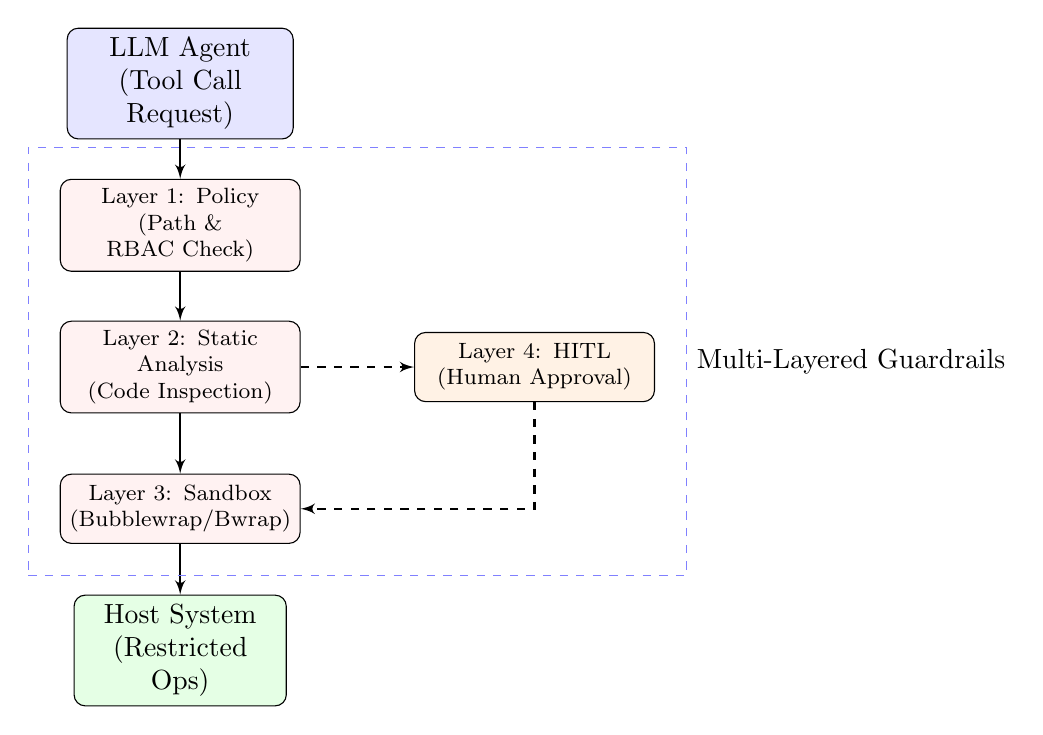
\begin{tikzpicture}[node distance=1.8cm, auto,
    block/.style={rectangle, draw, fill=blue!10, text width=7.5em, text centered, rounded corners, minimum height=3em},
    guard/.style={rectangle, draw, fill=red!5, text width=8em, text centered, rounded corners, minimum height=2.5em, font=\footnotesize},
    system/.style={rectangle, draw, fill=green!10, text width=7em, text centered, rounded corners, minimum height=3em},
    line/.style={draw, -latex', thick}]

    % Nodes
    \node [block] (agent) {LLM Agent \\ (Tool Call Request)};
    
    % Layer 1: Policy
    \node [guard, below of=agent] (policy) {Layer 1: Policy \\ (Path \& RBAC Check)};
    
    % Layer 2: Static Analysis
    \node [guard, below of=policy] (static) {Layer 2: Static Analysis \\ (Code Inspection)};
    
    % Layer 3: Sandbox
    \node [guard, below of=static] (sandbox) {Layer 3: Sandbox \\ (Bubblewrap/Bwrap)};
    
    % Layer 4: HITL
    \node [guard, right of=static, node distance=4.5cm, fill=orange!10] (hitl) {Layer 4: HITL \\ (Human Approval)};

    % System
    \node [system, below of=sandbox] (system) {Host System \\ (Restricted Ops)};

    % Paths
    \path [line] (agent) -- (policy);
    \path [line] (policy) -- (static);
    \path [line] (static) -- (sandbox);
    \path [line] (sandbox) -- (system);
    
    % HITL connection
    \path [line, dashed] (static) -- (hitl);
    \path [line, dashed] (hitl) |- (sandbox);

    % Legend or grouping
    \node[draw, dashed, blue!50, fit=(policy) (static) (sandbox) (hitl), inner sep=0.4cm, label=right:Multi-Layered Guardrails] (group) {};

\end{tikzpicture}

}
\caption{Multi-layered guardrail architecture for structural containment.}
\label{fig:guardrail_arch}
\end{figure}

\subsection{Layer 1: The "No-Shell" Execution Model}
Raw shell execution (\texttt{/bin/sh -c}) is structurally vulnerable because it conflates data and code. \texttt{llm-cli} adopts a "No-Shell" model where system operations are restricted to a specialized \texttt{execute\_python} tool. By executing Python code via \texttt{subprocess.run(args, shell=False)}, we eliminate shell-injection vectors. The agent must express intent in a structured programming language (Python), which is amenable to deterministic static analysis.

\subsection{Layer 2: Static Analysis and AST Inspection}
The generated code is parsed into an Abstract Syntax Tree (AST) before execution. The system applies a whitelist-based security scanner that traverses the tree using a \texttt{NodeVisitor} pattern. Specifically, we target:
\begin{itemize}
    \item \textbf{Module Blocking:} Prevents \texttt{import} of modules such as \texttt{os, socket, pty, ctypes}, and \texttt{requests} to block low-level OS access and unauthorized networking.
    \item \textbf{Function Sinks:} Blocks dangerous built-ins such as \texttt{eval(), exec(), getattr(),} and \texttt{\_\_import\_\_}.
    \item \textbf{Shell Injection Prevention:} Specifically inspects \texttt{subprocess} calls to ensure \texttt{shell=True} is never used, enforcing a strict separation between executable and arguments.
\end{itemize}

\subsection{Layer 3: Path Guardrails and Resource Limits}
All file-related operations are restricted to a designated workspace. We implement \textbf{Path Guardrails} that resolve symbolic links and verify that all targets reside within the allowed directory. 
Furthermore, we apply \textbf{OS-level Resource Limits} (\texttt{rlimit}):
\begin{itemize}
    \item \textbf{Memory:} Capped (e.g., 1GB) to prevent memory-exhaustion attacks.
    \item \textbf{CPU Time:} Timeouts per execution to mitigate infinite loops.
\end{itemize}

\subsection{Layer 4: Entropy-Based Secret Detection}
To prevent credential leaks to LLM providers, we monitor the \textbf{Shannon Entropy} ($H$) of the agent's output. High-entropy strings often correlate with cryptographic keys or session tokens.
\begin{equation}
H(X) = -\sum_{i=1}^{n} P(x_i) \log_2 P(x_i)
\end{equation}
We apply a heuristic threshold. When detected, these strings are automatically redacted before the tool-call response is returned to the model context.

\subsection{Layer 5: Linux Sandboxing (Bubblewrap)}
The final containment is provided by \textbf{Bubblewrap} (\texttt{bwrap}), which utilizes Linux namespaces to create an unprivileged environment:
\begin{itemize}
    \item \textbf{Filesystem Isolation:} Private, empty \texttt{/tmp} and \texttt{/home}.
    \item \textbf{Network Isolation:} The \texttt{--unshare-all} flag ensures the sandbox has no network interface.
    \item \textbf{Process Isolation:} No visibility of host-system processes (\texttt{/proc} is re-mounted).
\end{itemize}

\section{Evaluation}
We evaluated the framework's performance and effectiveness using a benchmark suite of 30 test cases, comprising 22 adversarial patterns (including obfuscated and reflection-based attacks) and 8 benign code samples.

\subsection{Containment Effectiveness}
Table \ref{tab:mitigation} summarizes the detection results for the Static Analysis layer (Layer 2).

\begin{table}[htbp]
\caption{Static Analysis Effectiveness ($n=30$)}
\begin{center}
\begin{tabularx}{\columnwidth}{|l|C|C|}
\hline
\textbf{Category} & \textbf{Count} & \textbf{Detection Rate} \\
\hline
Direct OS/Shell Access & 6 & 83.3\% \\
Obfuscation \& Reflection & 6 & 83.3\% \\
Networking \& Exfiltration & 4 & 75.0\% \\
File System Traversal & 3 & 100.0\% \\
Python Internals Access & 3 & 0.0\% \\
\hline
\textbf{Overall Adversarial} & \textbf{22} & \textbf{72.7\%} \\
\hline
\textbf{Benign (False Positive)} & \textbf{8} & \textbf{0.0\%} \\
\hline
\end{tabularx}
\label{tab:mitigation}
\end{center}
\end{table}

The evaluation indicates that while the static analyzer is effective at blocking common injection vectors (e.g., \texttt{os.system}), it did not detect certain advanced reflection techniques such as \texttt{object.\_\_subclasses\_\_()} or access via \texttt{globals()}. Additionally, direct use of \texttt{subprocess.Popen} without the \texttt{shell=True} flag was permitted by the current AST rules, although spawning a shell process would still be restricted by the sandbox.

These results emphasize the importance of a \textbf{Defense-in-Depth} approach. The 27.3\% of adversarial patterns that bypassed static analysis were successfully contained by \textbf{Layer 5 (Bubblewrap Sandboxing)}, which physically prevents network access and host filesystem modifications regardless of the code structure. By combining fast static filtering with robust OS-level isolation, the architecture achieves a balance of performance and security.

\subsection{Performance Latency}
Latency was measured on a system running WSL2 (AMD Ryzen 5 8540U, 16GB RAM). The results (Table \ref{tab:guardrail_perf}) show that the total security overhead remains minimal.

\begin{table}[htbp]
\caption{Guardrail Performance Metrics (Measured)}
\begin{center}
\begin{tabular}{|l|c|}
\hline
\textbf{Metric} & \textbf{Latency (ms)} \\
\hline
AST Analysis (Layer 2) & 0.04 \\
Secret Detection (Layer 4) & 0.01 \\
Sandboxed Exec Overhead (Layer 5) & 2.63 \\
\hline
\textbf{Total Security Overhead} & \textbf{2.68} \\
\hline
\end{tabular}
\label{tab:guardrail_perf}
\end{center}
\end{table}

The total overhead ($\approx$2.7ms) represents a small fraction of the time typically required for LLM inference (often ranging from 500ms to several seconds). This suggests that deterministic security guardrails can be implemented with negligible impact on the overall responsiveness of the agent.

\section{Conclusion}
Securing autonomous agents requires a transition from behavioral "alignment" toward structural, multi-layered guardrails. By combining a "No-Shell" model, AST inspection, and OS-level sandboxing, our framework provides a robust foundation for safe tool execution. This Phase 1 architecture ensures system integrity, establishing the environment for Phase 2, which addresses behavioral anomalies through Zero-Trust monitoring.

\begin{thebibliography}{00}
\bibitem{mcp2024} Anthropic, ``Model Context Protocol (MCP) Specification,'' 2024. [Online]. Available: https://modelcontextprotocol.io/
\bibitem{owasp2023} OWASP, ``Top 10 for Large Language Model Applications v1.1,'' 2023. [Online]. Available: https://owasp.org/www-project-top-10-for-large-language-model-applications/
\bibitem{nist2020zt} S. Rose, O. Borchert, S. Mitchell, and S. Connelly, ``Zero Trust Architecture,'' \textit{NIST Special Publication 800-207}, 2020.
\bibitem{mamba2023} A. Gu and T. Dao, ``Mamba: Linear-Time Sequence Modeling with Selective State Spaces,'' \textit{arXiv preprint arXiv:2312.00752}, 2023.
\bibitem{greshake2023not} K. Greshake, R. Abdelnabi, S. Mishra, C. Endres, T. Holz, and M. Fritz, ``Not what you've signed up for: Compromising Real-World LLM-Integrated Applications with Indirect Prompt Injection,'' \textit{arXiv preprint arXiv:2302.12173}, 2023.
\bibitem{masood2024sandboxed} A. Masood, ``The Sandboxed Mind: Principled Isolation Patterns for Prompt-Injection-Resilient LLM Agents,'' 2024. [Online]. Available: https://medium.com/@adnanmasood/the-sandboxed-mind-principled-isolation-patterns-for-prompt-injection-resilient-llm-agents-c14f1f5f8495
\bibitem{agentdojo2024} E. Debenedetti et al., ``AgentDojo: A Dynamic Environment to Evaluate Prompt Injection Attacks and Defenses for LLM Agents,'' \textit{arXiv preprint arXiv:2406.13352}, 2024.
\bibitem{perez2022ignore} F. Perez and I. Ribeiro, ``Ignore Previous Instructions: Prompt Injection Attacks on LLMs,'' \textit{arXiv preprint arXiv:2211.09527}, 2022.
\bibitem{ando2026zerotrust} Y. Ando, ``Zero-Trust Architecture for MCP-Based AI Agents: Continuous Identity and Behavioral Monitoring,'' \textit{TechRxiv}, 2026.
\bibitem{ando2026pqc} Y. Ando, ``Post-Quantum Workload Identity and Long-Term Audit Integrity for MCP-Based AI Agents,'' \textit{TechRxiv}, 2026.
\end{thebibliography}

\end{document}